\documentclass[class=article, crop=true]{standalone}
\usepackage{subcaption}
\usepackage[subpreambles=true]{standalone}
\usepackage{tikz}
\usepackage{amssymb}
\usepackage{amsmath}
\usetikzlibrary{arrows.meta, positioning}

\begin{document}

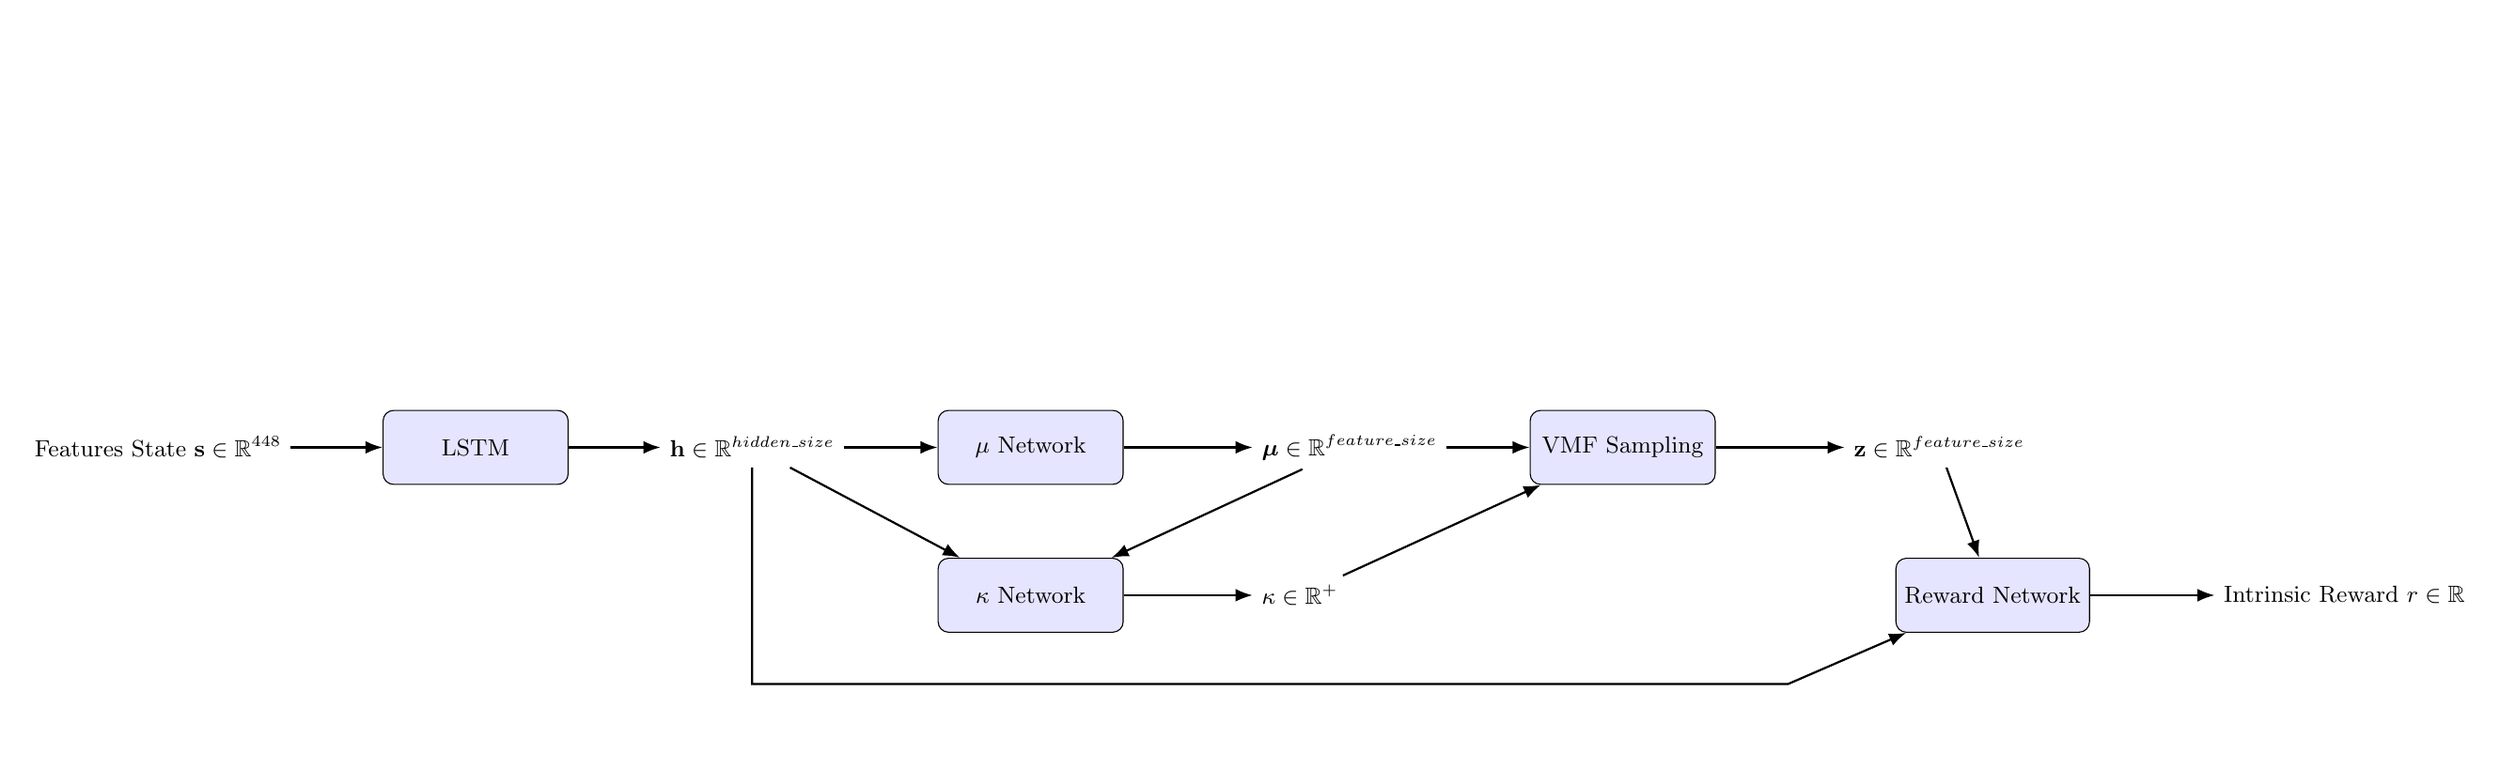
\begin{tikzpicture}[
    op/.style={rectangle, draw, rounded corners, text centered, minimum height=1cm, minimum width=2.5cm, font=\small, fill=blue!10},
    tensor/.style={font=\small},
    arrow/.style={-{Latex}, thick}
]

% Adjusted background to accommodate lower arrow
\fill[white] (-13.2, -4.2) rectangle (18.1, 5.7);

% Input state
\node[tensor, anchor=east] (state) at (-10, 0) {Features State $\textbf{s} \in \mathbb{R}^{448}$};

% LSTM
\node[op] (lstm) at (-7.5, 0) {LSTM};
\node[tensor, anchor=west] (hidden) at (-5, 0) {$\textbf{h} \in \mathbb{R}^{hidden\_size}$};

% Mu network branch
\node[op] (mu_net) at (0, 0) {$\mu$ Network};
\node[tensor, anchor=west] (mu) at (3, 0) {$\boldsymbol{\mu} \in \mathbb{R}^{feature\_size}$};

% Kappa network branch (moved slightly higher)
\node[op] (kappa_net) at (0, -2.0) {$\kappa$ Network};
\node[tensor, anchor=west] (kappa) at (3, -2.0) {$\kappa \in \mathbb{R}^+$};

% VMF sampling
\node[op] (vmf) at (8, 0) {VMF Sampling};
\node[tensor, anchor=west] (z) at (11, 0) {$\textbf{z} \in \mathbb{R}^{feature\_size}$};

% Reward network (moved slightly higher)
\node[op] (reward_net) at (13, -2.0) {Reward Network};
\node[tensor, anchor=west] (reward) at (16, -2.0) {Intrinsic Reward $r \in \mathbb{R}$};

% Connections with direct arrows
\draw[arrow] (state) -- (lstm);
\draw[arrow] (lstm) -- (hidden);
\draw[arrow] (hidden) -- (mu_net);
\draw[arrow] (hidden) -- (kappa_net);
\draw[arrow] (mu_net) -- (mu);
\draw[arrow] (mu) -- (vmf);
\draw[arrow] (mu) -- (kappa_net);
\draw[arrow] (kappa_net) -- (kappa);
\draw[arrow] (kappa) -- (vmf);
\draw[arrow] (vmf) -- (z);
\draw[arrow] (z) -- (reward_net);
% Modified path for hidden to reward_net to go under kappa_net
\draw[arrow] (hidden) -- ++(0,-3.2) -- ++(14,0) -- (reward_net);
\draw[arrow] (reward_net) -- (reward);

\end{tikzpicture}

\end{document}